\section{Context} 

As defined by the Human Genome Variation Society\footnote{https://hgvs-nomenclature.org/stable/recommendations/DNA/inversion/} (HGVS), inversions are sequence changes where, compared to a reference sequence, more than one nucleotide replacing the original sequence is the reverse complement of the original sequence. They are a category of genomic structural variations (SVs), defined as alterations in the DNA that affect more than 50 base pairs (bp). They may delete, insert, duplicate, invert, or move genomic sequences \cite{eslami_rasekh_discovery_2017} (see Figure \ref{fig:svs}). 

\begin{figure}[h]

  \centering
    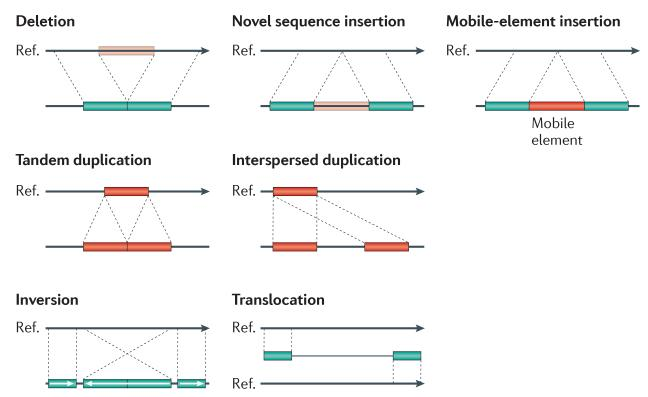
\includegraphics[width=250px]{svs.jpg}

  \caption{Outline of different SV-archetypes.}
  \label{fig:svs}
\end{figure}

They are often generated by non-allelic homologous recombination (NAHR) between inverted repeats, but they can also be originated by double-strand break repair mechanisms, like non-homologous end joining (NHEJ), or replication-based mechanisms mediated by microhomology, like fork stalling and template switching \cite{puig_human_2015}. Although inversions constitute only a small fraction of SVs across various organisms, ranging from 0.5\% to 7\% \cite{hu_unravelling_2024}, they can span over 100 Mb and collectively account for up to 10\% of the genome, holding considerable functional and evolutionary significance. \\


Inversions were first identified in 1917 by Alfred Sturtevant \cite{sturtevant_case_1921}, who found out that they act as suppressors of recombination between chromosomes. Since then, inversions have been increasingly drawing attention, due to their crucial role in driving genome evolution, as well as to their link to the evolutionary processes of many species. In fact, it was eventually discovered that suppressed recombination among genes within an inversion can lead to largely independent genome evolution between derived and ancestral arrangements, providing opportunities for divergence and speciation \cite{faria_evolving_2019}. Inversions thus facilitate genomic isolation, which can lead to the formation of novel genotypes and phenotypes, contributing to the genetic diversity we can observe today. \\

However, inversions are not only related to evolution: they are involved in the development of several diseases, as will be shown in Chapter 2. In fact, a recent study shows that the contribution of chromosomal inversions to phenotypic diversity can even affect brain development and lead to neurological disorders \cite{wang_chromosomal_2023}.

\section{Inversions detection}

Due to their significance, the challenge of detecting inversions has been widely addressed. The first methods developed to this scope, such as cytogenetics or approaches based on polymerase chain reaction (PCR), were labor‐intensive and lacked resolution, which limited their effectiveness \cite{hu_unravelling_2024}. With the advent of high-throughput next-generation sequencing (NGS), large-scale population studies of inversions finally became possible, enabling the discovery of polymorphic inversions and their association with phenotypic traits.
Additionally, highly effective, long‐read DNA sequencing technologies such as PacBio HiFi sequencing or Oxford Nanopore duplex sequencing now allow to generate sequencing reads between 10  kb and 2  Mb. These long reads can span repetitive and complex genomic regions, thus making identifying inversions a more straightforward task. Despite all this technological progress, inversions still remain one of the most underascertained forms of structural variation in human and non-human primate genomes, limiting our understanding of their significance in evolution \cite{porubsky_recurrent_2020}. The main challenge here continues to be the precise determination of inversion breakpoints.

\section{Project}

The scope of this thesis is to present an algorithm designed to detect the presence of genomic inversions from long-read sequencing data using sample-specific strings (which will be defined in detail in Chapter 2) to determine the breakpoints. The practical experimentation will use a \texttt{Python} implementation of the algorithm, in combination with the SVDSS \cite{denti_svdss_2023} tool, that will also be implemented in the code and will help detecting the number, position, and length of the sample-specific strings. \\
\\
Chapter 2 will present the necessary preliminaries to understand how the algorithm works, including the definitions used throughout the thesis and the biological background that underlies inversions, other than their practical biological consequences. \\
Chapter 3 will explain the algorithm in detail, including pseudocode and a complete theoretical analysis. This chapter will address, among other things, time and space complexity and proof of correctness.\\
Chapter 4 will focus on the practical experimentation, explaining the \texttt{Python} implementation of the code and the use of the SVDSS tool. The results will be presented, summarized, and commented upon.

\bigskip
\bigskip

